\section{Implementación del sistema Odoo}

\subsection{Configuración inicial}
\begin{indentedsubsection}
La implementación de la plataforma para Perú Flores Travel Agency Tours Operador E.I.R.L. se realiza bajo la modalidad Odoo Online (SaaS), lo que permite desplegar una solución centralizada en la nube accesible desde cualquier dispositivo móvil o computadora de escritorio. En esta etapa inicial se procedió a la creación del entorno de trabajo, definiendo la base de datos principal, la zona horaria y la configuración de una única moneda de trabajo: Dólares (USD), establecida por solicitud expresa de la cliente/gerencia para el cobro a turistas extranjeros. Se activaron los módulos de CRM, Ventas y Encuestas, preparando la estructura necesaria para la carga de datos maestros.
\end{indentedsubsection}

\begin{figure}[h!]
    \centering
    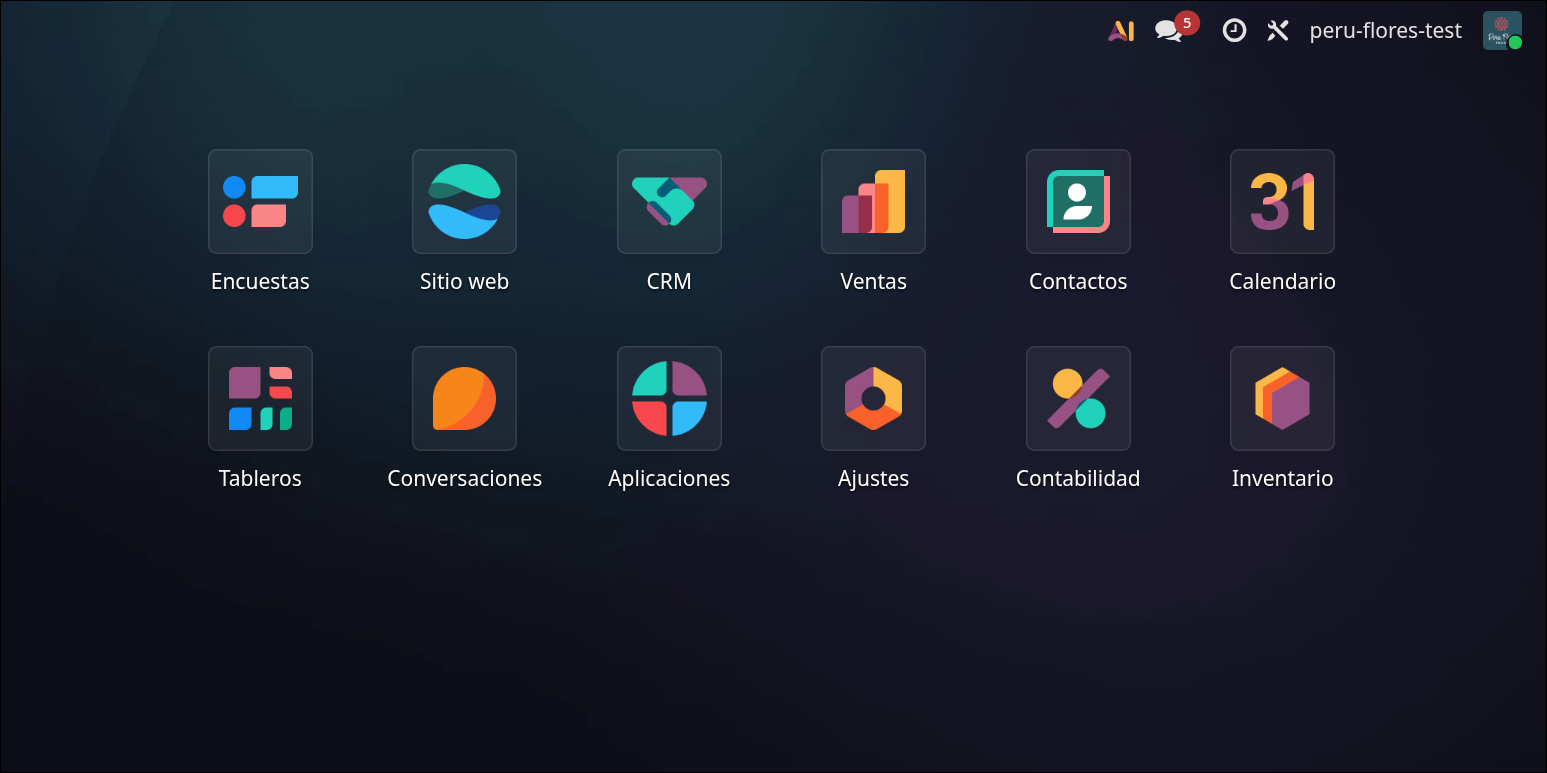
\includegraphics[width=0.9\textwidth]{assets/captura-configuracion-inicial-odoo-peruflores.png}
    \caption{Captura de la configuración inicial en Odoo Online}
\end{figure}

\subsection{Implementación del módulo CRM (Gestión turística y proveedores)}
\begin{indentedsubsection}
El CRM se configuró como el núcleo para la centralización de la base de datos, reemplazando definitivamente el uso de libretas físicas y la dispersión de contactos en WhatsApp. Las acciones clave incluyen:
\end{indentedsubsection}

\begin{indentedsubsection}
La vista de lista permite a la gerencia revisar rápidamente todos los contactos activos (pasajeros y proveedores), mientras que la ficha de detalle consolida información puntual de cada registro, incluyendo datos de identificación, trazabilidad comercial y notas operativas. Esta estructura facilita tanto el seguimiento diario como la búsqueda histórica de información sin depender de cuadernos ni chats dispersos.
\end{indentedsubsection}

\begin{figure}[h!]
    \centering
    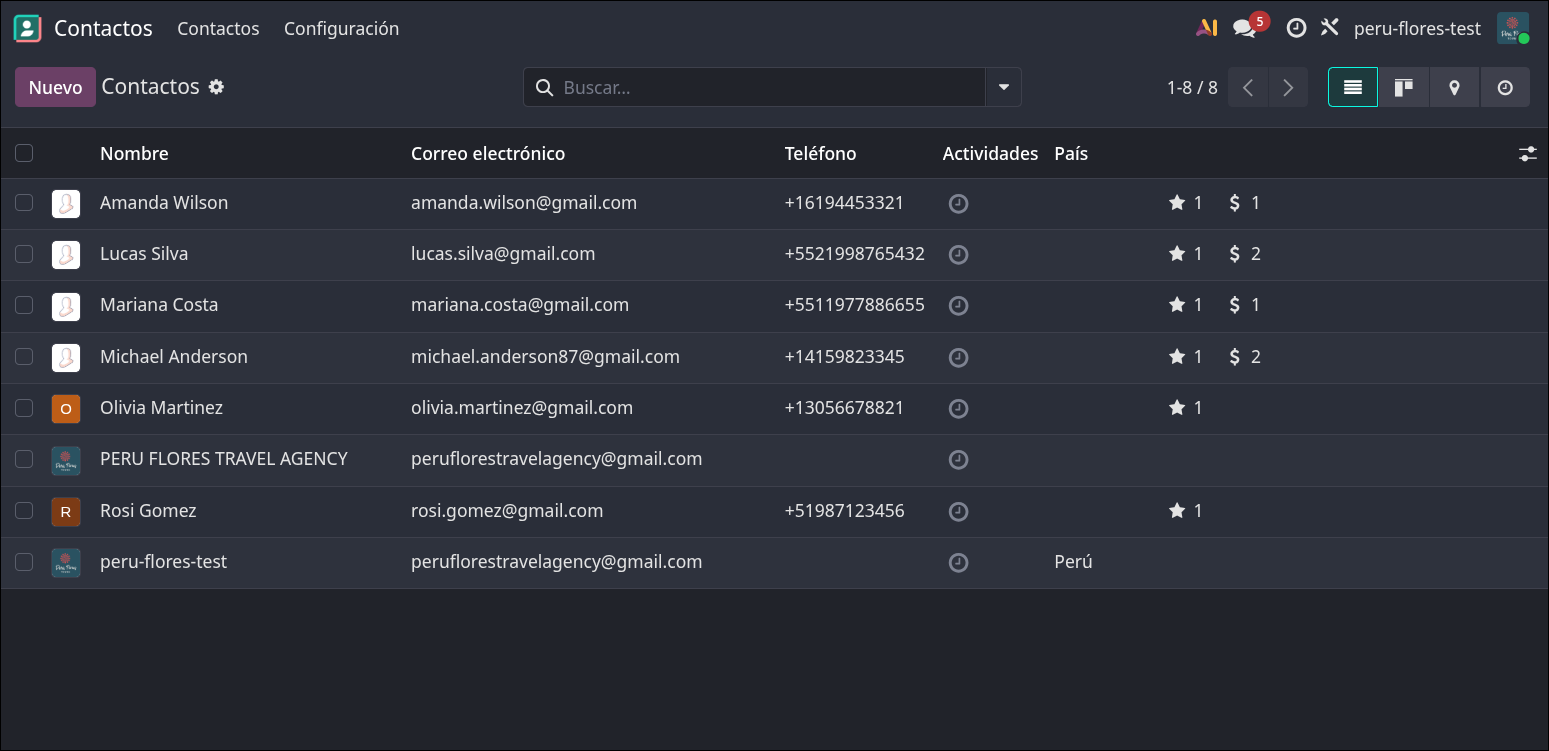
\includegraphics[width=0.9\textwidth]{assets/crm-lista-contactos-peruflores.png}
    \caption{Vista de lista de contactos en el módulo CRM}
\end{figure}

\begin{figure}[h!]
    \centering
    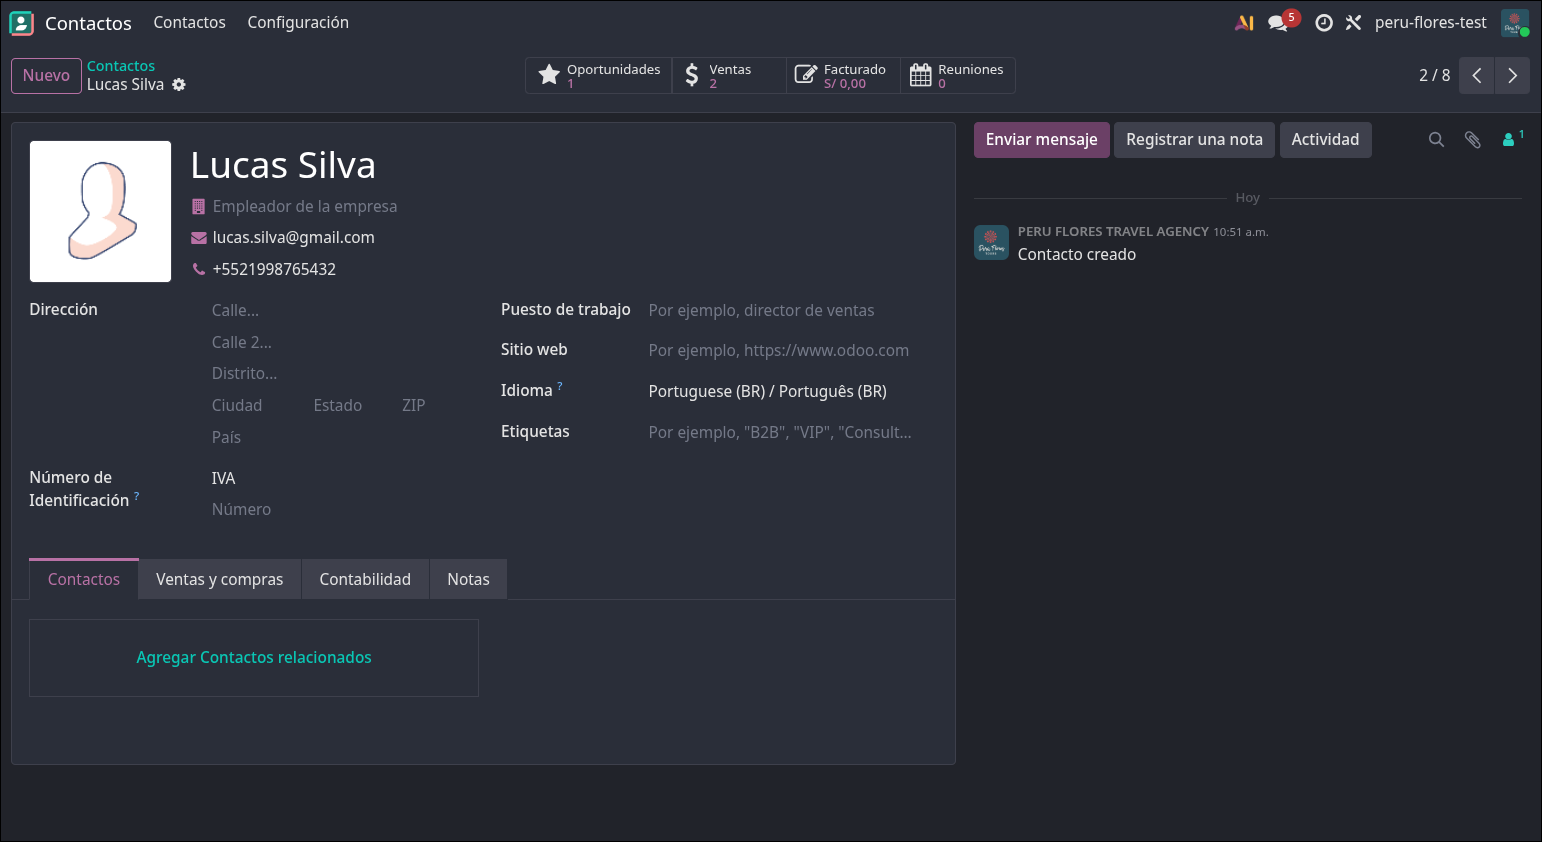
\includegraphics[width=0.9\textwidth]{assets/crm-detalle-contacto-peruflores.png}
    \caption{Vista de detalle de contacto en el módulo CRM}
\end{figure}

\begin{indentedsubsection}
\begin{itemize}
    \item \textbf{Ficha centralizada de contactos:} creación de un directorio unificado tanto para pasajeros (PAX) como para la red de proveedores (guías, transportistas, hoteles).
    \item \textbf{Embudo de ventas (Pipeline):} configuración de un embudo con etapas claras adaptadas al proceso de la agencia (Nuevo, Calificado, Propuesta, Ganado) para dar seguimiento visual a cada prospecto internacional desde su primer contacto.
    \item \textbf{Historial de comunicaciones:} registro de notas internas y preferencias del cliente en una sola pantalla, permitiendo a la gerencia saber exactamente qué se le ofreció a un turista sin tener que revisar chats antiguos.
\end{itemize}
\end{indentedsubsection}

\begin{indentedsubsection}
El embudo de ventas permite visualizar en tiempo real el estado de cada oportunidad comercial y priorizar las acciones de seguimiento. Con esta vista, la gerencia identifica rápidamente cuántos leads se encuentran en negociación, cuántos ya recibieron propuesta y cuáles se han cerrado con éxito, mejorando la capacidad de respuesta frente a nuevos requerimientos.
\end{indentedsubsection}

\begin{figure}[h!]
    \centering
    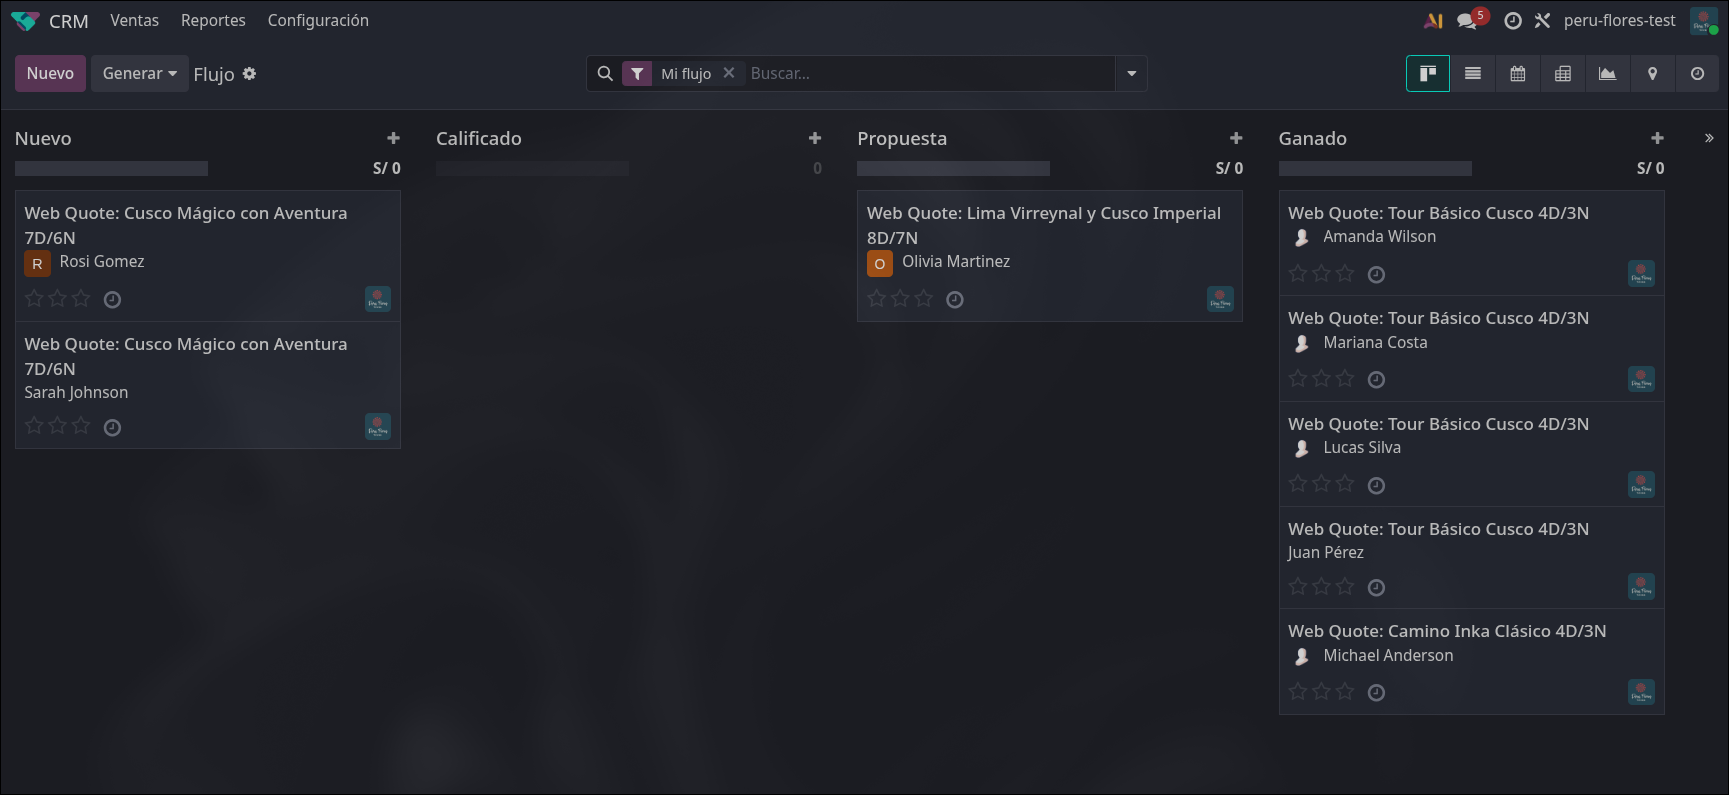
\includegraphics[width=0.92\textwidth]{assets/crm-embudo-ventas-leads-peruflores.png}
    \caption{Embudo de ventas (Pipeline) y gestión de leads en CRM}
\end{figure}

\subsection{Implementación del módulo de Ventas (Cotizador automatizado)}
\begin{indentedsubsection}
Para resolver el principal cuello de botella operativo (los cálculos manuales de los paquetes), se implementó el cotizador digital:

\begin{itemize}
    \item \textbf{Automatización de cálculos y prorrateos:} se configuró un catálogo de servicios tarifados (hoteles, trenes, ingresos, movilidad). El sistema calcula automáticamente la división de costos fijos (como el guía o el transporte) entre la cantidad de pasajeros, eliminando la necesidad de usar una calculadora externa.
    \item \textbf{Simulador de márgenes de ganancia:} se habilitó la función para que la gerencia pueda simular porcentajes de utilidad variables (ej. 15\%, 20\%, 30\%) dependiendo del perfil del turista, actualizando el precio final de venta al instante.
    \item \textbf{Generación de propuestas en PDF:} creación de plantillas formales con la identidad de Perú Flores. A solicitud expresa de la gerencia, se configuró el sistema para ocultar el desglose del IGV por ítem, mostrando un precio final limpio para no confundir al turista extranjero.
\end{itemize}
\end{indentedsubsection}

\begin{indentedsubsection}
La operación comercial en Ventas se estructuró para que la gerencia pueda gestionar todo el ciclo de una cotización desde una sola interfaz: creación del presupuesto, simulación de utilidad, envío al cliente por correo y generación del PDF final en formato profesional. Esto reduce retrabajo, evita errores de transcripción y acelera el tiempo de respuesta frente a solicitudes de cambios.
\end{indentedsubsection}

\begin{figure}[h!]
    \centering
    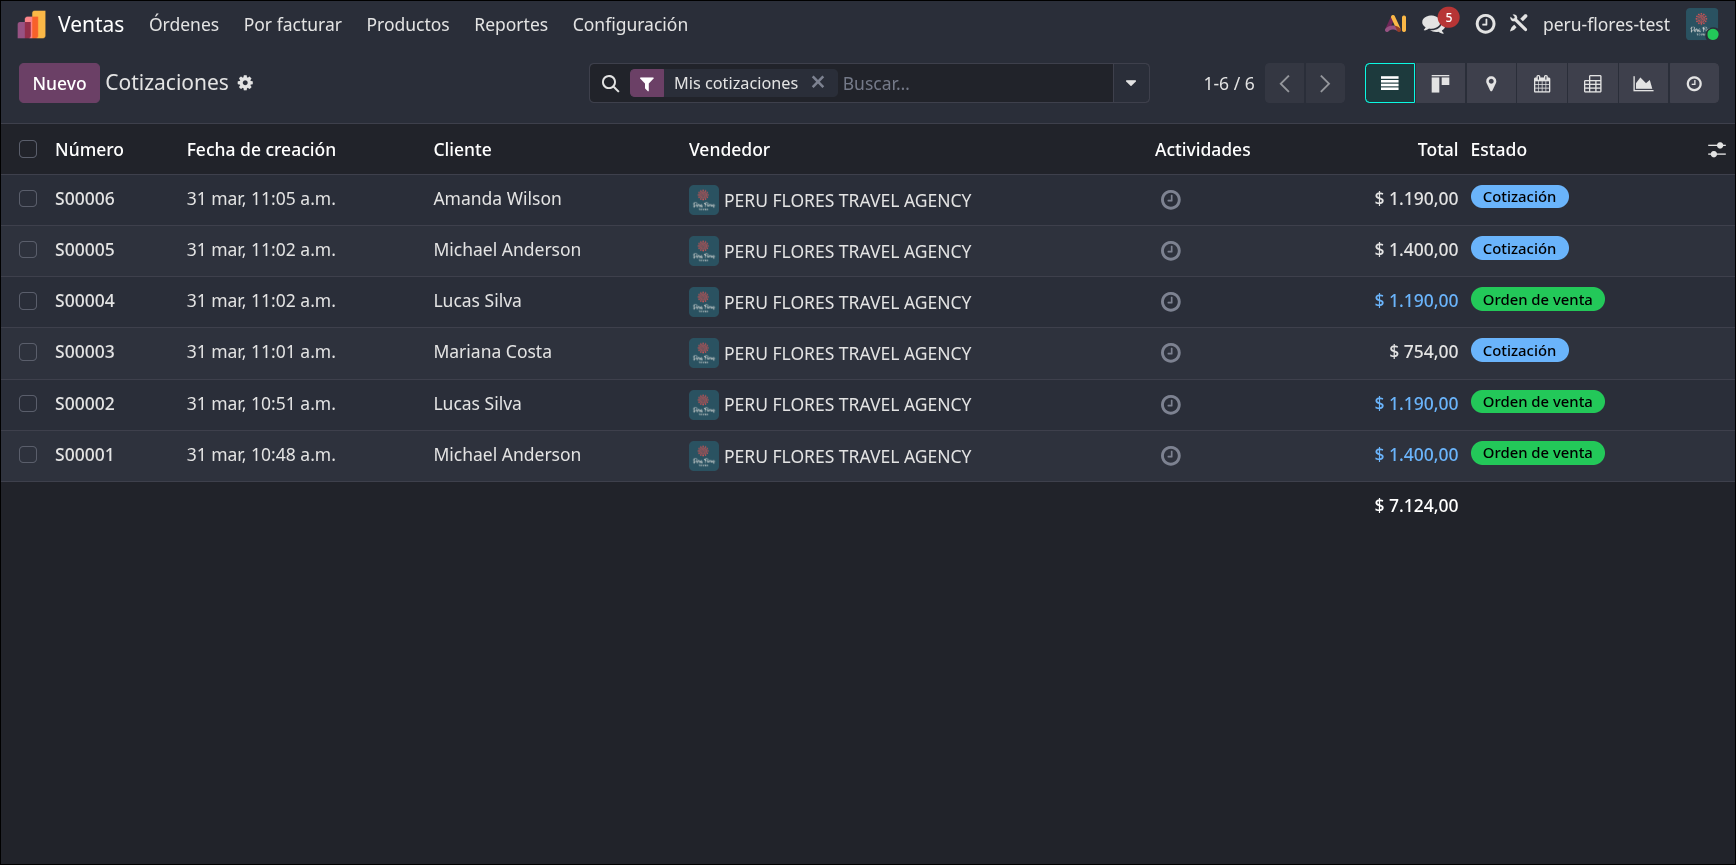
\includegraphics[width=0.92\textwidth]{assets/ventas-lista-cotizaciones-peruflores.png}
    \caption{Vista general de cotizaciones en el módulo de Ventas}
\end{figure}

\begin{figure}[h!]
    \centering
    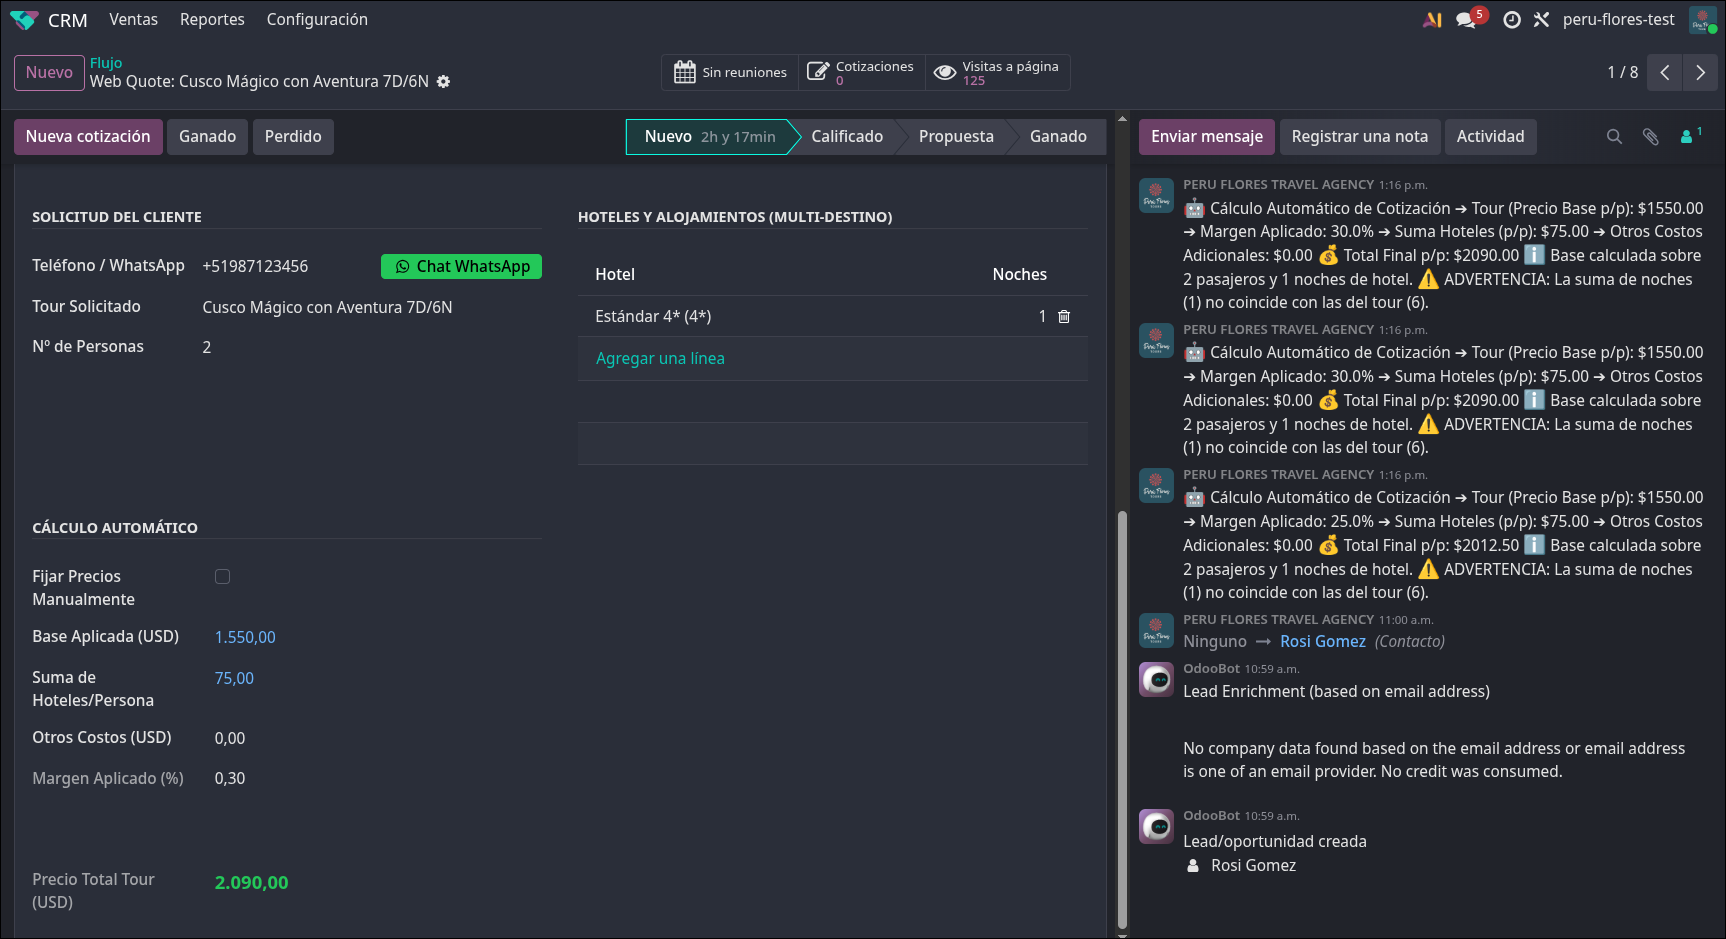
\includegraphics[width=0.92\textwidth]{assets/ventas-simulador-ganancias-peruflores.png}
    \caption{Automatización de cálculos y simulador de ganancias}
\end{figure}

\begin{indentedsubsection}
Como parte del flujo de cierre comercial, se habilitó la comunicación directa desde el propio sistema para enviar la propuesta al turista internacional sin salir de Odoo. De esta manera, cada cotización queda trazada con su historial de envío y versión de documento, fortaleciendo el control operativo y la formalidad comercial.
\end{indentedsubsection}

\begin{figure}[h!]
    \centering
    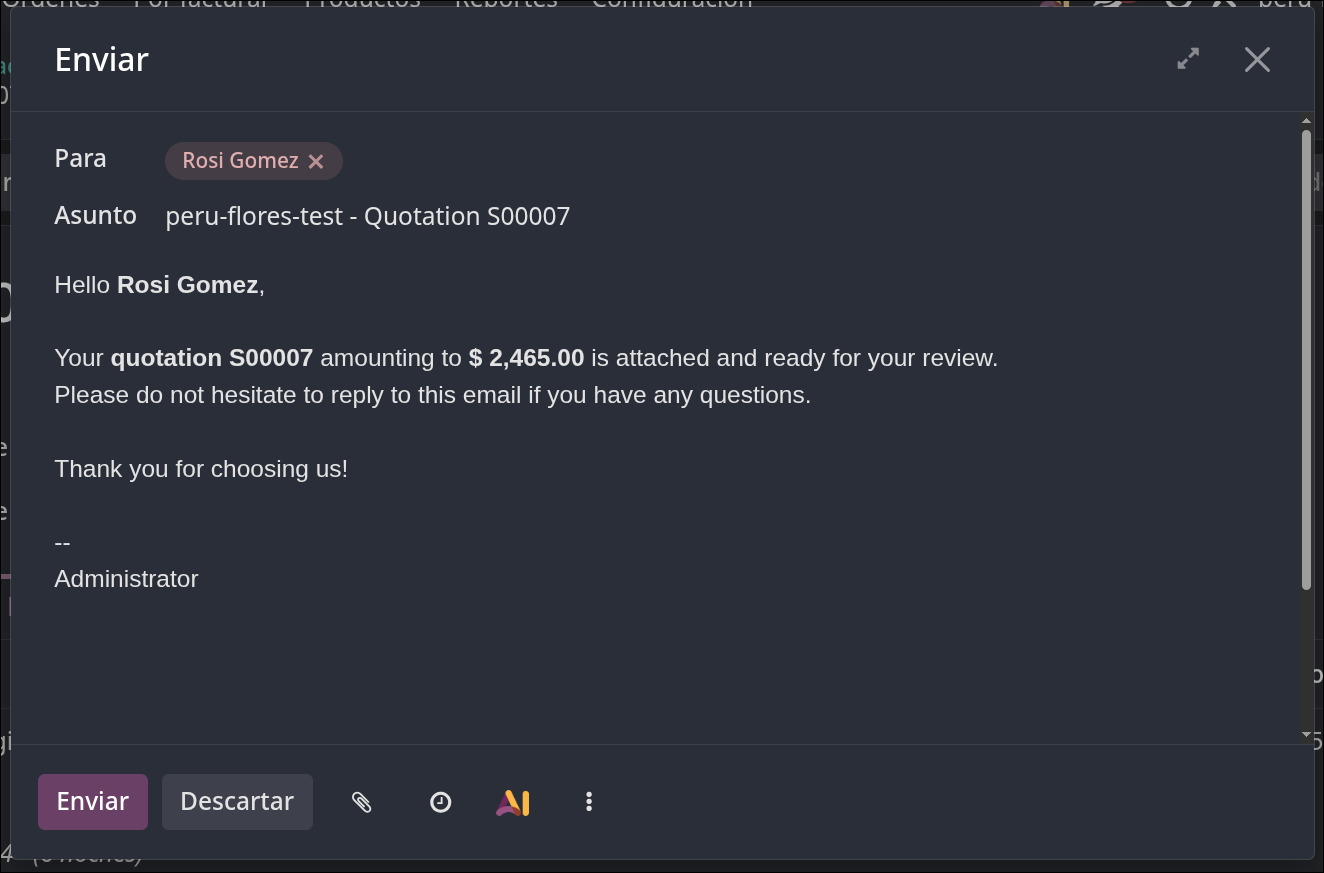
\includegraphics[width=0.88\textwidth]{assets/ventas-modal-correo-cotizacion-peruflores.png}
    \caption{Modal de envío por correo de la cotización}
\end{figure}

\begin{figure}[h!]
    \centering
    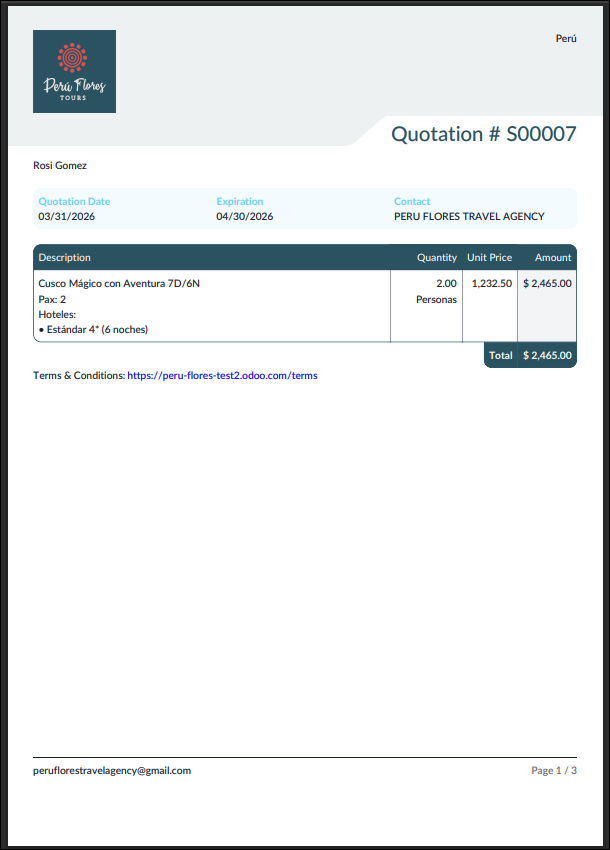
\includegraphics[width=0.4\textwidth]{assets/ventas-pdf-cotizacion-pagina-1-peruflores.png}
    \caption{Cotización generada en PDF - Página 1}
\end{figure}

\begin{figure}[h!]
    \centering
    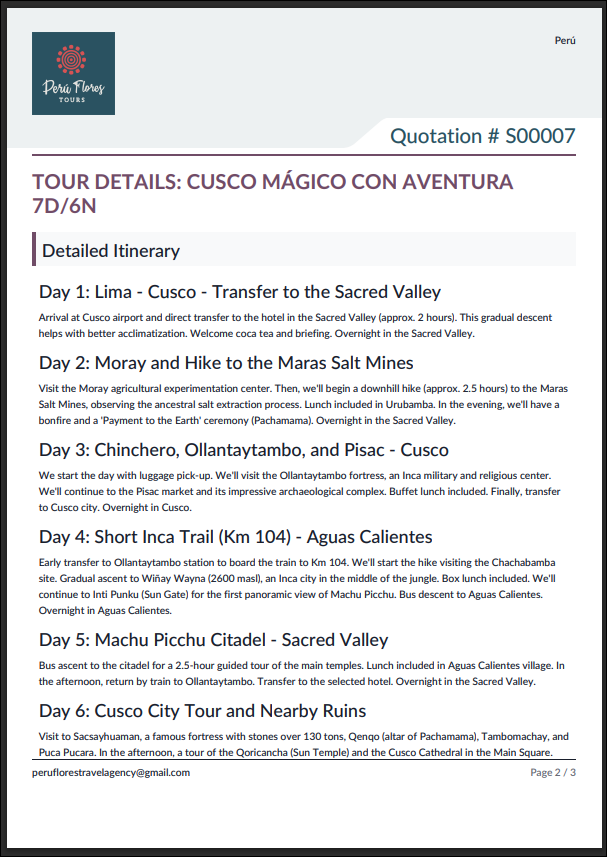
\includegraphics[width=0.4\textwidth]{assets/ventas-pdf-cotizacion-pagina-2-peruflores.png}
    \caption{Cotización generada en PDF - Página 2}
\end{figure}

\subsection{Gestión de cobros y pagos fraccionados}
\begin{indentedsubsection}
Se parametrizó el flujo de ventas para gestionar la realidad de cobranza de la agencia, la cual no suele recibir el 100\% del pago por adelantado:

\begin{itemize}
    \item \textbf{Registro de adelantos:} configuración para ingresar manualmente los abonos (pagos ``a cuenta'') que los clientes realizan a través de medios externos como Western Union o depósitos bancarios.
    \item \textbf{Control de saldos:} el sistema calcula y muestra de forma automática el ``saldo pendiente'' de cada pasajero, brindando a la gerencia un control exacto antes de proceder con la ejecución del paquete turístico.
\end{itemize}
\end{indentedsubsection}

\subsection{Implementación del módulo de Encuestas (Feedback Post-Servicio)}
\begin{indentedsubsection}
Para potenciar la reputación de la agencia y la mejora continua, se implementó el módulo de retroalimentación:

\begin{itemize}
    \item \textbf{Formularios de satisfacción:} diseño de una encuesta digital (replicando el formulario que la agencia ya validó en el pasado) para calificar del 1 al 10 el servicio de guías, transporte y atención general.
    \item \textbf{Automatización y ``Boca a boca'':} el envío de estas encuestas se realiza al finalizar el itinerario, consolidando testimonios valiosos que permiten auditar la calidad de los proveedores y generar material para futuras recomendaciones.
\end{itemize}
\end{indentedsubsection}

\begin{indentedsubsection}
La encuesta fue configurada para que el equipo pueda reutilizar una plantilla estándar por cada servicio concluido, manteniendo consistencia en los criterios de evaluación. Adicionalmente, la vista de resultados consolida métricas clave en un resumen visual que facilita la toma de decisiones sobre mejoras operativas y desempeño de proveedores.
\end{indentedsubsection}

\begin{figure}[h!]
    \centering
    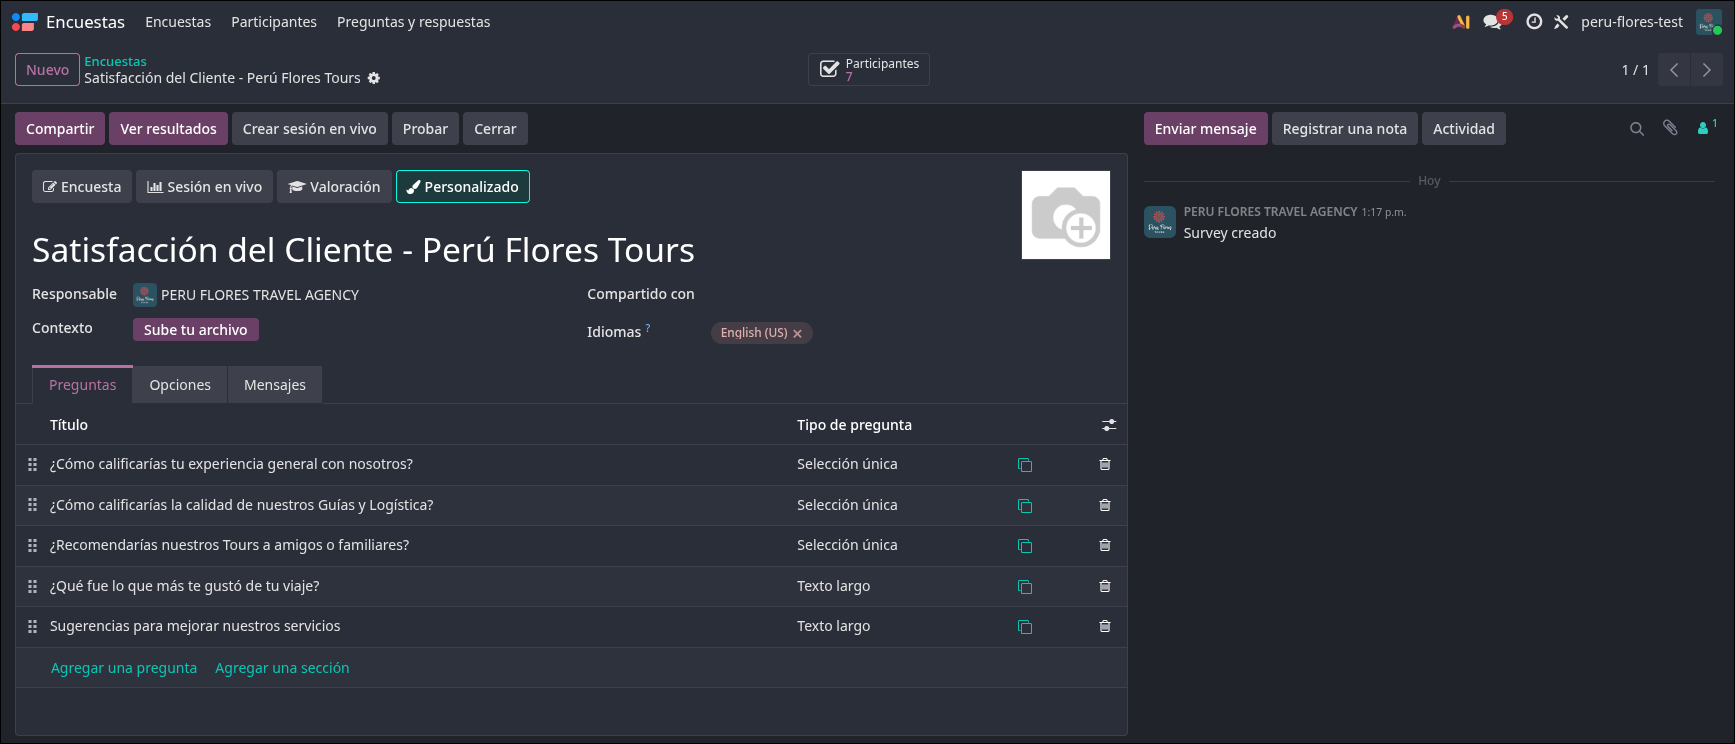
\includegraphics[width=0.9\textwidth]{assets/encuestas-formulario-feedback-peruflores.png}
    \caption{Formulario digital de encuesta post-servicio}
\end{figure}

\begin{figure}[h!]
    \centering
    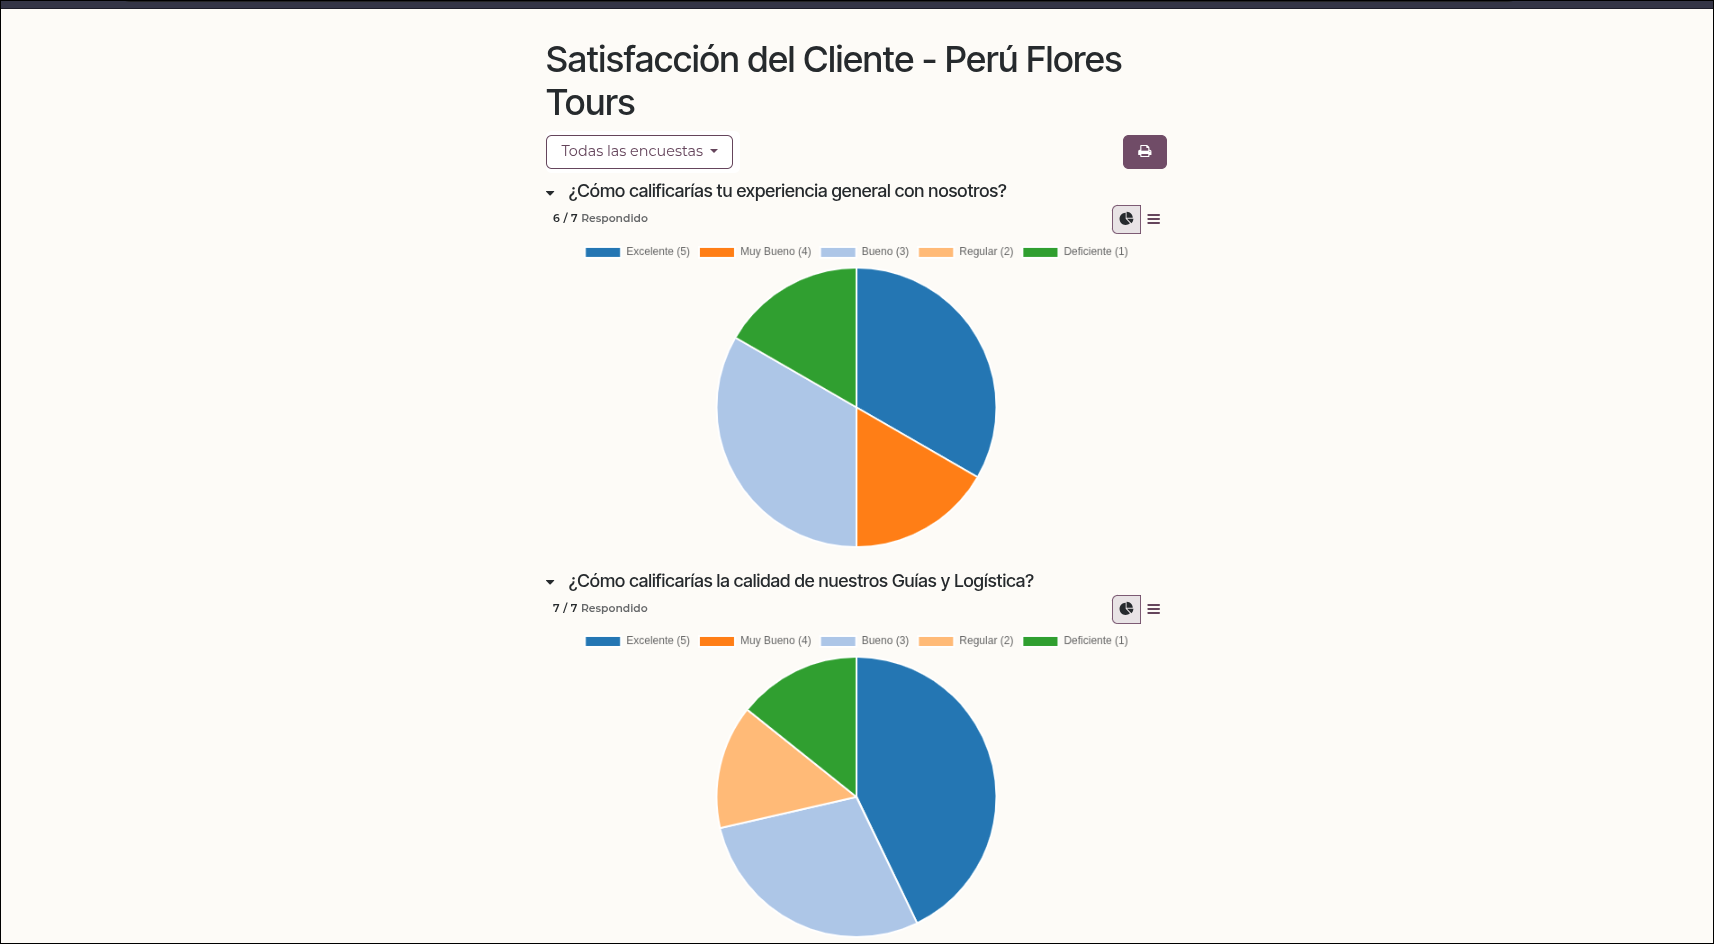
\includegraphics[width=0.9\textwidth]{assets/encuestas-resumen-resultados-peruflores.png}
    \caption{Resumen de resultados de encuestas de satisfacción}
\end{figure}

\subsection{Integración entre módulos y trazabilidad del sistema}
\begin{indentedsubsection}
La fortaleza de esta implementación radica en la interconexión. Un prospecto que ingresa al CRM se convierte en una oportunidad; desde esa misma pantalla se genera la cotización en Ventas con los precios automatizados. Una vez que el cliente acepta, se registra su adelanto por Western Union, y al finalizar el viaje, el sistema detona la Encuesta. La información fluye de manera ordenada sin requerir doble digitación en ningún momento.
\end{indentedsubsection}

\subsection{Mapa de procesos actual (con Odoo)}
\begin{indentedsubsection}
A continuación, se describe el flujo operativo resultante, ágil y centralizado:
\end{indentedsubsection}

\begin{figure}[h!]
    \centering
    \includegraphics[width=0.95\textwidth]{assets/mapa-procesos-actual-odoo-peruflores.png}
    \caption{Mapa de procesos actual con Odoo en Perú Flores}
\end{figure}

\begin{indentedsubsection}
\begin{itemize}
    \item \textbf{Captación y Registro:} el turista extranjero contacta por WhatsApp. La gerencia lo registra inmediatamente en el CRM de Odoo (desde su celular o computadora) creando una nueva Oportunidad.
    \item \textbf{Cotización Inmediata:} dentro de la oportunidad, se seleccionan los servicios (hotel, BTG, guía). Se aplica un margen de ganancia (ej. 25\%) y Odoo calcula el precio exacto por pasajero al instante. Se genera un PDF profesional (sin desglose de IGV) y se envía al cliente.
    \item \textbf{Confirmación y Adelanto:} el cliente acepta la propuesta y envía su depósito por Western Union. La gerencia registra en el sistema el pago ``a cuenta'', y Odoo actualiza automáticamente el saldo pendiente.
    \item \textbf{Ejecución del Tour:} la gerencia coordina la operación teniendo toda la información del cliente centralizada, sin depender de archivos de Excel aislados.
    \item \textbf{Cierre y Feedback:} al finalizar el servicio, se envía el enlace de la Encuesta de satisfacción. El cliente califica su experiencia, cerrando el ciclo comercial y dejando un registro histórico para su fidelización.
\end{itemize}
\end{indentedsubsection}
